\documentclass[12pt]{article}

%%%% PACKAGES %%%%

\usepackage{verbatim}
\usepackage{graphicx}
\usepackage[space]{grffile}
\usepackage[utf8]{inputenc}
\usepackage{cite}
\usepackage{etoolbox}
\patchcmd{\thebibliography}{\section*{\refname}}{}{}{}
\usepackage{hyperref}
\hypersetup{%
pdfborder = {0 0 0}
}
\usepackage{xcolor}
\usepackage{tikz}
\usepackage{amssymb}
\usepackage{listings}
\usepackage{mathtools}
\usepackage{amsmath}

%%%%%%%%

%%%% MACROS %%%%

\newcommand{\singlespace}{\vspace{5 mm}}
\newcommand{\doublespace}{\vspace{10 mm}}
\newcommand{\triplespace}{\vspace{15 mm}}

\newcommand{\ceil}[1]{\lceil#1\rceil}
\newcommand{\blank}{\sqcup}
\newcommand{\ti}[1]{\textit{#1}}
\renewcommand{\contentsname}{Contents}

%%%%%%%%

\begin{document}

%%%% LOGO %%%%

\begin{center}

\includegraphics[scale=1]{Images/tesiSCIENZE_TECNOLOGIE.jpg}
\end{center}

%%%%%%%%

%%%% TITLE %%%%

\begin{center}
\triplespace

\begin{Huge}
\textbf{Image classification with Random Forest}
\end{Huge}

\triplespace

\begin{Large}
Davide Franchi\\
\singlespace
960803
\end{Large}
\end{center}

%%%%%%%%

\newpage
\tableofcontents
\newpage
\section{Problem details}
The problem asks to classify images with 784 pixel, varying in $\{0, ..., 255\}$ each. Labels are in $\{0, ..., 9\}$ instead.\\
So the data points space is $\mathcal{X} = \{0, ..., 255\}^{784}$, while the label space is $\mathcal{Y} = \{0, ..., 9\}$.\\
The training set $S$ includes 60000 ground truths.\\\\
As the title of the report suggests, the classification is realized by a\\ Random Forest classifier: an ensemble of tree classifiers, which predict the label of a data point $x$ according to the one assigned to the leaf to which $x$ has been routed to from the root.\\
Each tree is learned trying to minimize the training error, computed by the 0-1 loss.
\newpage
\section{Implementation choices}
\subsection{Tree predictors}
Here is described the chosen structure for tree classifiers.\\
Let the trees be with maximum depth at most 10 and with test of the form $x[f] \le v$ in the internal nodes, where $f$ is a feature among a set of 25, chosen uniformly at random (without replacement).\\
So the implementation below provides binary tree classifiers.
\subsubsection{Training subset size}
Here is described the desired size of the training subsets to use for learning tree classifiers.\\
The class of tree classifiers on which the predictor will be picked up includes at most:
$$\sum_{i = 1}^{2^{10 + 1} - 1}\left(2e \cdot 25 \cdot 256 \cdot 10\right)^{i} \le \left(2e \cdot 25 \cdot 256 \cdot 10\right)^{2^{10 + 1}}$$
different predictors.\\
Indeed, fixed a number of nodes $1 \le i \le 2^{10 + 1} - 1$, there can be at most $0 \le j \le i$ internal nodes, each one with at most $25\cdot256$ different tests of the above form, and at most $i - j$ leaves, with at most 10 different labels each.\\
Using the upper bound ${i \choose k} \le \left(\frac{ei}{k}\right)^k$ over the $(i-1)$-th Catalan number, which counts the number of binary trees with $i$ nodes, $\left(2e \cdot 25 \cdot 256 \cdot 10\right)^{i}$ is an\\ upper bound for the number of tree predictors of this form with exactly $i$ nodes.\\\\
So, to bound the variance error of the tree classifier (chosen by trying to minimize the training error) over the chosen class, the number of "different" samples extracted from the training set $S$ for the learning of a predictor must be of the order of $\log \left(\left(2e \cdot 25 \cdot 256 \cdot 10\right)^{2^{10 + 1}}\right)$. "Different" means that $S$ could contain a given sample more than once and that is not a problem (it depends on the distribution over $\mathcal{X} \times \mathcal{Y}$), but picking exactly the same element from $S$ twice would not be helpful for the learning.\\
The chosen size is $\lfloor 2^{10 + 1} \log \left(2e \cdot 25 \cdot 256 \cdot 10\right)\rfloor = 26132$, which cannot be\\ increased anymore for time reasons.
\subsubsection{Training subset construction}
Here is described how the construction of each subset takes place and how is possible to achieve the desired size.\\
The extraction is computed uniformly at random, with replacement.\\ However, since duplicates are not helpful, they are discarded at the end of the whole extraction. To clarify once again the meaning of "duplicates": it is not helpful to include in a training subset a $sample_j \in S$ twice; however, if $S$ contains $sample_j, sample_{z \neq j}$ such that $sample_j = sample_z$ and they are both extracted they are both included of course.\\ Let $ext_i$ be the number of extractions performed for the $i-th$ training subset\\ $S^{(i)} \subseteq S$, used for the learning of the $i-th$ tree in the forest.\\
Since the probability of a sample of being chosen during the extraction of $S^{(i)}$ is $1 - \left(1 - \frac{1}{|S|}\right)^{ext_i}$ and since the expected number of unique elements of $S$ in each subset $S^{(i)}$ (so the cardinality of each $S^{(i)}$ of course) should be $26132$: 
$$ext_i = \log_{1 - \frac{1}{|S|}}\left(1 - \frac{26132}{|S|}\right) \approx 34312$$
Indeed:
$$E\left[\right|S^{(i)}\left|\right] = \sum_{j = 1}^{|S|} P\left(sample_j\ is\ chosen\right)$$
$$= \sum_{j = 1}^{|S|} \left(1 - \left(1 - \frac{1}{|S|}\right)^{ext_i}\right)$$
$$= \left| S \right|\left(1 - \left(1 - \frac{1}{|S|}\right)^{ext_i}\right)$$
Now, the above mentioned value for $ext_i$ is obtained by imposing\\ $E\left[\right|S^{(i)}\left|\right] = 26132$ as desired.\\\\
Moreover, $\forall i \neq j$, the probability of a sample of being chosen by both $S^{(i)}$ and $S^{(j)}$ is $\left( 1 - \left( 1 - \frac{1}{|S|} \right)^{34312} \right)^2 \approx 0.190$, by the independence of the drawn. This means that the expected percentage of elements of $S$ which appears in both the subsets is around 19 ($\approx 11400$ samples, only the $\approx 43,6\%$ of their size).
\newpage
\subsubsection{Leaves splitting}
Here is described how the training error is reduced and how the split of a leaf is performed.\\
The idea is to allow as many splits as possible, which are never harmful with 0-1 loss (as in the binary case). Indeed, let $v_i \ge 0$ be the number of votes for label $i$ in a given leaf $l$. The number of wrong predictions of $l$ over the training subset is given by:
$$\sum_{i=0}^9 v_i - \max(v_0, ..., v_9)$$
After the split this quantity is replaced by:
$$\left(\sum_{i=0}^9 v_i' - \max(v_0', ..., v_9')\right) + \left(\sum_{i=0}^9 v_i'' - \max(v_0'', ..., v_9'')\right)$$
where $v_i', v_i'' \ge 0$ and $v_i' + v_i'' = v_i$, $\forall i$.\\
The first one is greater than or equal to the second one iff:
$$\max(v_0, ..., v_9) \le \max(v_0', ..., v_9') + \max(v_0'', ..., v_9'')$$
and this inequality is clearly always true. Let $v_{i^*}$ be the maximum: either $v_{i^*}', v_{i^*}'' = v_{i^*} - v_{i^*}'$ are both the maximum on the right, or the right quantity is strictly greater than the left one.\\\\
So, to achieve the maximum number of splits, given a leaf $l$, let $S_l^{(i)}$ be the subset of data points $x$ of the $i$-th subset of the training set $S$, provided for the training of the $i$-th tree, routed to $l$. For each feature $f$ (among a set of 25 random features, chosen for the tree, which is random shuffled at each split to encourage diversity and decrease the bias error) consider the value $v$ which minimizes $\left| \left| \{ x \in S_l^{(i)}:\ x \left[ f \right] \le v \} \right| - \frac{\left| S_l^{(i)} \right|}{2} \right|$.\\
Then, pick the first one for which the above-mentioned $v$ is such that:
$$\alpha \frac{\left| S_l^{(i)} \right|}{2} \le \left| \{ x \in S_l^{(i)}:\ x \left[ f \right] \le v \} \right| \le (2 -\alpha) \frac{\left| S_l^{(i)} \right|}{2}$$
where the coefficient $\alpha$ is fixed and has been chosen as $\frac{9}{10}$. It is useful to usually stop the search in advance.\\
This choice is backed by the idea above and the fixed depth of the trees: the only way to maximize splits (with the intention of decreasing training error of course) is to play with breadth, routing as many samples as possible to both branches.\\
Trying over 10 trees, it has produced a minimum of 2045 and a maximum of 2047 nodes. Essentially, 10 complete binary trees.\\\\
Since $v$ lays in a tight range (only 256 possible values), the count of samples with given feature-value less than or equal to something can be speeded up by using bucket sort. Assuming a sequential execution of the algorithm, the bucket array can be declared once to save memory.\\
So, assuming to be $V$ the size of the range on which $v$ lays and $F$ the\\ number of features to examine at each split (which is 25 in this case), a split requires time $O(F(V + |S_l^{(i)}|))$ to select the test. The actual split of samples to $l_1, l_2$ can be done (with high probability) in time $O(|S_l^{(i)}|)$ by using sets implemented with hash-tables.\\
This implementation is fast for low depth nodes, which probably handle high $|S_l^{(i)}|$, and maybe a bit slow for the others. Anyway, it should be generally preferable.
\subsubsection{Label assignment}
The label is assigned to each leaf according to the majority of samples-labels routed to it. Ties are broken choosing the lowest label.
\subsection{Forest predictor}
The forest just starts with a given number of trees and grows one by one, when required, to speed up the test with different forest-sizes.\\
The prediction applies the same majority criteria used by single trees to assign leaves labels, among the predictions provided by the trees in the forest.
\newpage
\section{Experimental results}
The main experiment consists in growing a forest, looking for the dependence\\ between the test error of the forest predictor and the number of trees involved.\\
The growth has been stopped once reached a sort of "balance threshold": let $err(t)$ be the test error obtained by the current forest predictor involving $t$ trees and $best$ be the lowest test error obtained until now, then the experiment ends iff: $$\bigwedge_{i = t - att}^t \left(best - err(i) \le \epsilon\right)$$ to avoid fluctuations. The expectation is to see the error (always) decrease as the forest size increases of course.\\
The values chosen have been $\epsilon = 10^{-3}$ and $att = 2$.
\newpage
The result is qualitatively summarized in the following diagram (produced from a test set of size 10000):
\begin{center}
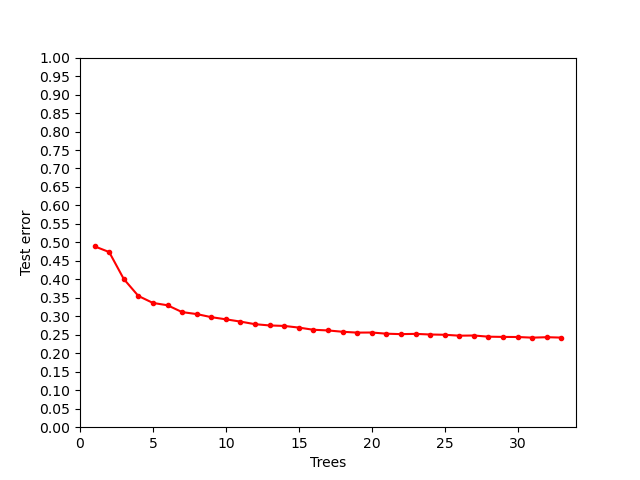
\includegraphics[width=1.3\textwidth]{Images/Test_error_diag.png}
\end{center}
So, that suggests an error of $\approx 24\%$ for random forest predictors (built as explained) with at least 30 trees.\\
Since a random classifier for this problem has a risk of the $90\%$, it does not seem to be so bad.
\newpage
Just to be confident, the diagram below shows the gap between the\\ previous curve and the one obtained by estimating the error of the predictor built by the algorithm with 5-fold cross validation, for forest of size $\le 10$ (for time reasons):
\begin{center}
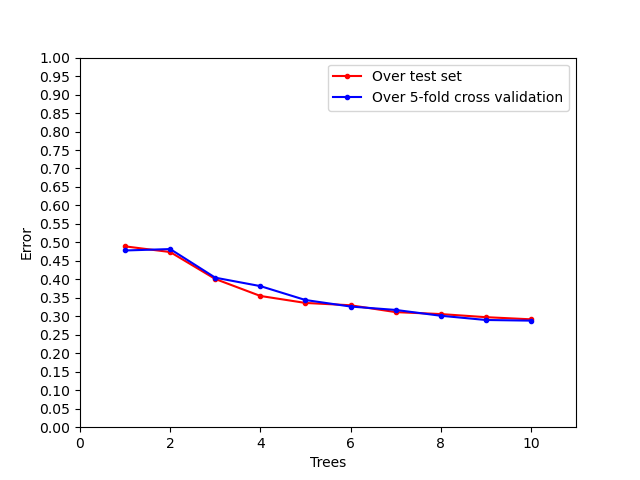
\includegraphics[width=1.3\textwidth]{Images/5_fold_diag.png}
\end{center}
Since the 5-fold cross validation from a training set of 60000 samples allows to estimate the quality of the predictor returned by the algorithm given an arbitrary training set of fixed size $\left(\frac{4}{5}\right)60000 = 48000$, this diagram suggests that starting from 48000 or 60000 training samples should be the same.\\
For each fold, the value of $ext_i$ explained in 2.1.2 is computed considering $|S| = 48000$ instead of 60000 of course.
\newpage
Instead, the real values of the main experiment (actually just a subset) are:\\

\begin{table}[!h]
\centering

\begin{tabular}{|p{0.50\textwidth}|p{0.50\textwidth}|}
\hline
\begin{center}
1
\end{center}
& \begin{center}
0.4893
\end{center}
\\
\hline
\begin{center}
2
\end{center}
& \begin{center}
0.4739
\end{center}
\\
\hline
\begin{center}
3
\end{center}
& \begin{center}
0.4010
\end{center}
\\
\hline
\begin{center}
4
\end{center}
& \begin{center}
0.3551
\end{center}
\\
\hline
\begin{center}
5
\end{center}
& \begin{center}
0.3362
\end{center}
\\
\hline
\begin{center}
13
\end{center}
& \begin{center}
0.2753
\end{center}
\\
\hline
\begin{center}
23
\end{center}
& \begin{center}
0.2525
\end{center}
\\
\hline
\begin{center}
33
\end{center}
& \begin{center}
0.2424
\end{center}
\\
\hline
\end{tabular}
\end{table}
The only "nonconformist" seems to be the forest with 2 trees, which does not improve the single tree so much (while in general adding a tree to a little forest seems to significantly reduce the error).\\
Indeed, having 10 possible predictions and breaking ties by choosing the\\ lowest one, every time the correct label is high, the only way for the forest with 2 trees to predict correctly is to have either two identical (correct) predictions, or the wrong one higher than the correct.\\
Actually, as shown by the following diagram (built over test error differences of 10 independent constructions):
\begin{center}
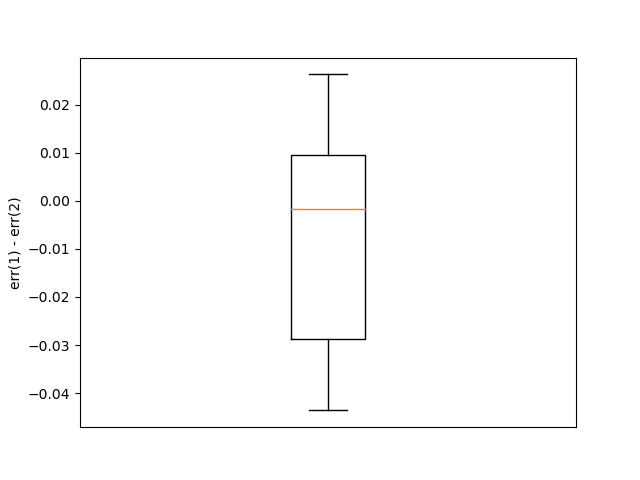
\includegraphics[width=1.3\textwidth]{Images/Forest2_diag.png}
\end{center}
having two trees instead of one in general does not seem to lead to any\\ improvement.
\newpage
The following diagram instead shows the relation between the training error and the test error of a forest of 20 trees (which does not seem to produce an error so different from the bigger ones and allows saving computations), built from training set of different sizes (obtained by randomly subsampling without replacement the original training set):
\begin{center}
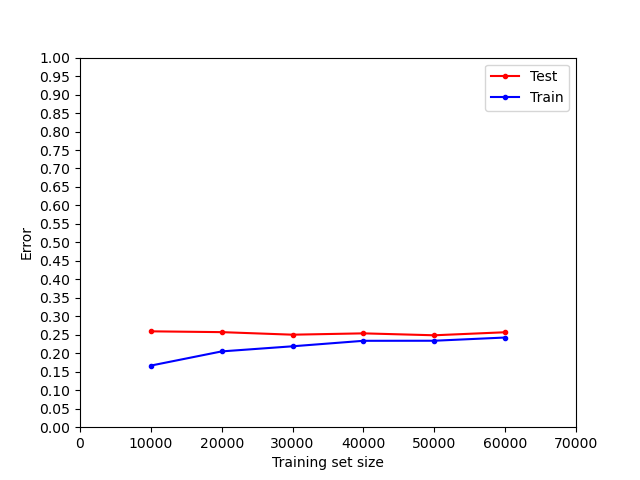
\includegraphics[width=1.3\textwidth]{Images/Test_vs_train_diag.png}
\end{center}
According to this, the algorithm seems to not overfit with training sets of size at least 40000. However, this is actually not as surprising as could seem, since, according to what has been said in 2.1.2 (talking about the\\ construction of the training subset), for a fixed tree a notable part of the whole training set $S$ remains unknown, if this is big enough, and the training error is computed among all the samples of $S$.\\
However, it could underfit, since the restrictions imposed to the structure of the tree classifiers to save computations (and to be able to provide a training subset big enough to bound the variance error over the single trees) have reduced a lot the size of the class, increasing the bias error.\\\\
Pay attention: according to what has been said in 2.1.1 about the desired training subset size and to the fact that the formula for $ext_i$ described in 2.1.2 does not make sense for training set of size $\le 26132$, the training subsets for the case 10000 and 20000 have been chosen by picking the whole training set randomly shuffled.\\\\
Both the construction time and the prediction time grow linearly with the number of trees added to the forest of course, so it has been chosen to not show any diagram about them.
\subsection{Time and equipment}
The whole experiment required about 4 hours over a laptop with:
\begin{enumerate}
\item Processor: Intel Core i7-9750H CPU @ 2.60GHz x 12
\item Ram: 31,3 GiB
\item OS: Ubuntu 18.04.4 LTS (64 bit)
\end{enumerate}
The code has been implemented using python 3.8.3.\\\\
The whole project (except the folders containing the training set and the test set) has been loaded to:\\
\url{https://github.com/Deido182/Image_classification}
\newpage
\section{Copyright}
I declare that this material, which I now submit for assessment, is entirely my own work and has not been taken from the work of others, save and to the extent that such work has been cited and acknowledged within the text of my work. I understand that plagiarism, collusion, and copying are grave and serious offenses in the university and accept the penalties that would be imposed should I engage in plagiarism, collusion or copying. This assignment, or any part of it, has not been previously submitted by me or any other person for assessment on this or any other course of study.
\end{document}